\newpage
\section{Ejemplos}


\subsection{Ejemplo 1}
En este ejemplo consideramos como espacio de entrada $X$ el
{\em espacio de Hilbert\/} $\mathbb{R}^2$, con su estructura
can\'onica de espacio con producto interno.
As\'\i\ es que $X$ tiene bastante estructura y es mucho m\'as que
un conjunto no vac\'\i o.

\smallskip\noindent
En el espacio de entrada $X=\mathbb{R}^2$ consideramos la data:
$$
P_1=(1,0)\,,\quad
P_2=(0,1)\,,\quad
P_3=(-1,0)\,,\quad
P_4=(0,-1)\,,\qquad
Z_0=(0,0)\,.
$$

\begin{center}
% from \url{http://tex.stackexchange.com/questions/61316/draw-a-plot-with-point}
\begin{tikzpicture}[x=1cm,y=1cm]

 \draw[latex-latex, thin, draw=gray] (-2,0)--(2,0) node [right] {$x$}; % l'axe des abscisses
 \draw[latex-latex, thin, draw=gray] (0,-2)--(0,2) node [above] {$y$}; % l'axe des ordonnées


\draw[fill] (1,0) circle [radius=0.05];
\node [below] at (1,0) {$P_1$};


\draw[fill] (0,1) circle [radius=0.05];
\node [below] at (0,1) {$P_2$};

\draw[fill] (-1,0) circle [radius=0.05];
\node [below] at (-1,0) {$P_3$};

\draw[fill] (0,-1) circle [radius=0.05];
\node [below] at (0,-1) {$P_4$};

\draw[fill,red] (0,0) circle [radius=0.05];
\node [red, below] at (0,0) {$Z_0$};


% to ensure that the points are being properly centered:
\draw [dotted, gray] (-3,-3) grid (3,3);
%\node [red] at (0,0) {\textbullet};

\end{tikzpicture}
\end{center}



Claramente no es posible separar linealmente el dato $Z_0$
de los datos $P_k, k=1, \ldots, 4$.
Separar linealmente significa aqu\'\i\ separar $Z_0$ de los $P_k$
mediante un subespacio lineal (i.e., vectorial) de $\mathbb{R}$,
esto es mediante una recta que pase por el origen, dejando $Z_0$
a un lado y los $P_k$ al otro.
\smallskip\noindent
Como espacio de caracter\'\i sticas queremos utilizar el
{\em espacio de Hilbert\/} $\mathbb{R}^3$, con su estructura
can\'onica de espacio con producto interno.

\smallskip\noindent
Para ponernos en el contexto de lo discutido en este ensayo,
queremos considerar $\mathbb{R}^3$ como un espacio de funciones
apropiado, lo que en este caso quiere decir que se trata de
funciones que podemos describir un\'\i vocamente mediante 3
par\'ametros $(a,b,c)\in\mathbb{R}^3$.

\smallskip\noindent
Hay muchas opciones posibles.
Examinemos la m\'as simple, que consiste en considerar el conjunto
${\rm\bf Aff}(\mathbb{R}^2,\mathbb{R})$ de las transformaciones afines:
$$
f_{(a,b,c)}:\mathbb{R}^2\to\mathbb{R}\,,\qquad
f_{(a,b,c)}(x,y):= ax+by+c\,,\quad (x,y)\in\mathbb{R}^2\,.
$$
De este modo, a cada punto $(a,b,c)\in\mathbb{R}^3$ corresponde una
y s\'olo una transformaci\'on af\'\i n
$f_{(a,b,c)}\in{\rm\bf Aff}(\mathbb{R}^2,\mathbb{R})$.

\smallskip\noindent
N\'otese que para $(x,y)\in\mathbb{R}^{\textcolor{red}{2}}$ se tiene:
\begin{align*}
f_{\lambda(a,b,c)+\mu(a',b',c')}(x,y)
&= f_{(\lambda a + \mu a',\lambda b + \mu b',\lambda c + \mu c')}(x,y) \\
&= (\lambda a + \mu a')x + (\lambda b + \mu b')y + (\lambda c + \mu c') \\
&= \big( \lambda a x + \lambda b y + \lambda c \big) +
   \big( \mu a' x + \mu b' y + \mu c' \big) \\
&= \lambda \big( a x + b y + c \big) + \mu \big( a' x + b' y + c' \big) \\
&= \lambda f_{(a,b,c)}(x,y) + \mu f_{(a',b',c')}(x,y)\,.
\end{align*}
Luego, la identificaci\'on $(a,b,c)\mapsto f_{(a,b,c)}$ define un
isomorfismo\footnote{Revisar en Sec. \label{sec:def} la definici\'on de isomorfismo.} entre los espacios vectoriales $\mathbb{R}^3$ y
${\rm\bf Aff}(\mathbb{R}^2,\mathbb{R})$:
$$
\mathbb{R}^3 \cong {\rm\bf Aff}(\mathbb{R}^2,\mathbb{R})
\subset \mathfrak{F}(\mathbb{R}^2,\mathbb{R})
= \mathbb{R}^{\mathbb{R}^2}\,.
$$

\smallskip\noindent
Ahora consideraremos una aplicaci\'on $\Phi$ ``sacada de la manga'',
pero que, como se ver\'a, constituye una inmersi\'on apropiada
para construir el kernel en este ejercicio:
$$
\Phi:\mathbb{R}^2\to\mathbb{R}^3 \cong 
{\rm\bf Aff}(\mathbb{R}^2,\mathbb{R})\,,\qquad
\Phi(\xi,\eta):= (\xi,\eta, -2\xi^2-2\eta^2+1)\,,\quad 
(\xi,\eta)\in\mathbb{R}^2\,.
$$
Bajo la acci\'on de $\Phi$ los datos $P_k$ y $Z_0$ se transforman en:
\begin{equation*}
Z_0\mapsto W_0 = (0,0,1)\,,\qquad
\begin{cases}
P_1\mapsto Q_1 = (1,0,-1)\,, & \\
P_2\mapsto Q_2 = (0,1,-1)\,, & \\
P_3\mapsto Q_3 = (-1,0,-1)\,, & \\
P_4\mapsto Q_4 = (0,-0,-1)\,. &
\end{cases}
\end{equation*}


\tdplotsetmaincoords{60}{110}
\begin{center}
\begin{tikzpicture}[scale=2,tdplot_main_coords]

\coordinate (O) at (0,0,0);

\draw[thick] (-2,0,0) -- (2,0,0) node [anchor=north east] {$x$};
\draw[thick] (0,-2,0) -- (0,2,0) node[anchor=north west]{$y$};
\draw[thick] (0,0,-2) -- (0,0,2) node[anchor=south]{$z$};



\draw[fill] (1,0,-1) circle [radius=0.05];
\node [below] at (1,0,-1) {$Q_1$};


\draw[fill] (0,1,-1) circle [radius=0.05];
\node [below] at (0,1,-1) {$Q_2$};


\draw[fill,red] (0,0,1) circle [radius=0.05];
\node [below,red] at (0,0,1) {$W_0$};

\draw[fill,red] (1,0,0) circle [radius=0.05];
\node [below] at (1,0,0) {$(1,0,0)$};


\draw[fill,red] (0,0,-1) circle [radius=0.05];
\node [below] at (0,0,-1) {$(0,0,-1)$};


\end{tikzpicture}
\end{center}


Observando la geometr\'\i a de la situaci\'on, es evidente que
en $\mathbb{R}^3 \cong {\rm\bf Aff}(\mathbb{R}^2,\mathbb{R})$
el punto $W_0$ es f\'acilmente separable de los puntos $Q_k$
por infinitos subespacios lineales de $\mathbb{R}$, esto es,
por planos (de dimensi\'on 2) {\em que pasan por el origen\/}.
Uno de estos subespacios, por ejemplo, es el plano $E_{(1,1,2)}$
de $\mathbb{R}^3$ que viene dado por:
$$
E_{(1,1,2)}:\qquad
[x,y,z]^T \begin{bmatrix} 1 \\ 1 \\ 2 \end{bmatrix}
= x+y+2z = 0\,,\qquad 
[x,y,z]^T\in\mathbb{R}^3 \cong {\rm\bf Aff}(\mathbb{R}^2,\mathbb{R})\,.
$$
En efecto, el punto $W_0$ est\'a ``por encima'' de $E_{(1,1,2)}$
y los puntos $Q_k$ ``por debajo''.

\smallskip\noindent
La inmersi\'on $\Phi$ permite determinar los puntos
$(\xi,\eta)\in\mathbb{R}^2$ tales que:
$$
(\xi,\eta) \overset{\Phi}{\longmapsto} 
(\xi,\eta,-2\xi^2-2\eta^2+1) = (x,y,z)\in E_{(1,1,2)}\,.
$$
Dado que $E_{(1,1,2)}$ viene dado por $x+y+2z=0$, de la definici\'on de
$\Phi$ resulta que los correspondientes puntos $(\xi,\eta)\in\mathbb{R}^2$
deben satisfacer la 
$$
\xi + \eta - 4\xi^2 - 4\eta^2 + 2 = 0\,,\qquad
(\xi,\eta)\in\mathbb{R}^2\,.
$$
Evidentemente, esta curva algebraica se puede escribir tambi\'en en la
forma:
$$
\left( \xi-\frac18 \right)^2 + \left( \eta-\frac18 \right)^2
= \frac38\,,\qquad (\xi,\eta)\in\mathbb{R}^2\,,
$$
que corresponde a una circunferencia $\Gamma$ en $\mathbb{R}^2$
con centro en $(-1/8,-1/8)=(-0.125,\,-0.125)$ y radio 
$\sqrt{3/8}=0.612372436\dots$.
Luego, como era previsible, la circunferencia $\Gamma$ encierra
al punto $Z_0$ y los puntos $P_k$ est\'an por fuera de $\Gamma$.
Por su parte, la inmersi\'on $\Phi$ transforma
el exterior de $\Gamma$ en el semi-espacio que est\'a
``por debajo'' del plano $E_{(1,1,2)}$, 
el interior de $\Gamma$ en el semi-espacio que est\'a
``por encima'' del plano $E_{(1,1,2)}$, y
la circunferencia $\Gamma$ en el plano $E_{(1,1,2)}$.

\smallskip\noindent
Utilizando la inmersi\'on $\Phi$ se observa que el kernel
$K\big( (\xi_1,\eta_1),\,(\xi_2,\eta_2) \big)$ viene dado por:
\begin{align*}
K\big( (\xi_1,\eta_1),\,(\xi_2,\eta_2) \big)
&= \left\langle k_{(\xi_1,\eta_1)},\,k_{(\xi_2,\eta_2)}
   \right\rangle_{\mathbb{R}^3} \\
&= \big\langle \Phi(\xi_1,\eta_1),\,\Phi(\xi_2,\eta_2)
   \big\rangle_{\mathbb{R}^3} \\
&= \left\langle \big[\xi_1,\eta_1,-2\xi_1^2-2\eta_1^2+1\big]^T\,,\;
   \big[\xi_2,\eta_2,-2\xi_2^2-2\eta_2^2+1\big]^T
   \right\rangle_{\mathbb{R}^3} \\
&= \xi_1^2 + \eta_1^2 + \left(-2\xi_1^2-2\eta_1^2+1\right)^2 +
   \xi_2^2 + \eta_2^2 + \left(-2\xi_2^2-2\eta_2^2+1\right)^2
\end{align*} 





Una interesante tarea consistir\'\i a en averiguar cu\'ales son
las curvas (algebraicas, por supuesto) de nivel del kernel $K$.
Tal ejercicio deber\'\i a comenzar por graficar dichas curvas
mediante Mathematica (TM), por ejemplo.
No abordamos este {\em divertimento\/}, por ahora.

\subsection{Ejemplo 2}

{\color{red} 
El ejemplo que sigue es bastante confuso.
Convendr\'\i a ``enderezarlo'' ---matem\'atica-, gramatical-,
y estil\'\i sticamente--- con base en el desarrollo del
Ejemplo 1.

\smallskip\noindent
Se tiene un espacio de entrada $X=\mathbb{R}^2$ donde sus elementos
no son linealmente separables. 
Se desea llevar los elementos de $X$ a un espacio de caracter\'\i sticas
$H=\mathbb{R}^3$ mediante una aplicaci\'on 
$\Phi:X\to H$, donde los elementos en $H$ s\'\i\ sean linealmente
separables. 
Entonces se tiene:
\begin{eqnarray*}
\Phi: \mathbb{R}^2=X &\hookrightarrow &H=\mathbb{R}^3 \\
x=(x_1,y_2) &\rightarrow & \Phi(x):=(x_1^2,\sqrt{2}x_1 x_2,x_2^2)
\end{eqnarray*}
Tambi\'en se denomina $\Phi(x)=k_x$.

%% \begin{figure}[ht!]
%% \centering
%% \includegraphics[width=100mm]{ejemplo.jpg}
%% \caption{Ejemplo de kernel}
%% \label{ejemplo}
%% \end{figure}

\smallskip\noindent
El espacio de Hilbert $H$ est\'a dado por las funciones
$\{f:\mathbb{R}^2 \rightarrow \mathbb{R}\}$ definidas como:
{\bf (Dudo mucho que esto tenga pies y cabeza)} 
\begin{eqnarray*}
f: \mathbb{R}^2 &\rightarrow& \mathbb{R} \\
x &\rightarrow& f(x) = \langle (a,b,c), \Phi(x)\rangle \\
& & f(x) = a x_1^2 + b x_2 ^2 + c \sqrt{2} x_1 x_2
\end{eqnarray*}
con $a,b,c\in\mathbb{R}$, donde ahora $f\in H$ puede ser representado
por:
\begin{equation}
f= (a,b,c)
\end{equation}
Para este ejemplo la funci\'on de kernel:
\begin{eqnarray*}
K: X \times X &\rightarrow &H=\mathbb{R}^3 \\
    (x,y) &\rightarrow & K(x,y)
\end{eqnarray*}
se define como:
\begin{align*}\smash[t]
K(x,y):
&= k_x(y)
 = \langle k_x, k_y \rangle
 = \langle \Phi(x), \Phi(y) \rangle \\
&= \left\langle \big( x_1^2,\sqrt{2}x_1 x_2,x_2^2 \big)\,,\;
                \big( y_1^2,\sqrt{2}y_1 y_2,y_2^2 \big) \right\rangle \\
&= x_1^2 y_1^2 + 2x_1x_2y_1 y_2 + x_2^2 y_2^2
 = \big(\langle x,y \rangle \big)^2\,,\qquad x,y\in X=\mathbb{R}^2\,.
\end{align*}
}



\begin{figure}[ht!]
\centering
\includegraphics[width=100mm]{img/ejemplo.jpg}
\caption{Ejemplo de kernel}
\label{ejemplo}
\end{figure}
